
%%%%%%%%%%%%%%%%%%%%%%%%%%%%%%%%%%%%%%%%%%%%%%%%%%%%%%%%
%
% Copyright (c) 2003-2009 by University of Queensland
% Earth Systems Science Computational Center (ESSCC)
% http://www.uq.edu.au/esscc
%
% Primary Business: Queensland, Australia
% Licensed under the Open Software License version 3.0
% http://www.opensource.org/licenses/osl-3.0.php
%
%%%%%%%%%%%%%%%%%%%%%%%%%%%%%%%%%%%%%%%%%%%%%%%%%%%%%%%%


\chapter{Models}
\label{MODELS CHAPTER}

The following sections give a breif overview of the model classes and their corresponding methods.

\section{Stokes Problem}
The velocity \index{velocity} field $v$ and pressure $p$ of an incompressible fluid \index{incompressible fluid} is given as the solution of the Stokes problem\index{Stokes problem}
\begin{equation}\label{Stokes 1}
-\left(\eta(v\hackscore{i,j}+ v\hackscore{i,j})\right)\hackscore{,j}+p\hackscore{,i}=f\hackscore{i}-\sigma\hackscore{ij,j}
\end{equation}
where $\eta$ is the viscosity, $F\hackscore{i}$ defines an internal force \index{force, internal} and $\sigma\hackscore{ij}$ is an intial stress \index{stress, initial}. We assume an incompressible media:
\begin{equation}\label{Stokes 2}
-v\hackscore{i,i}=0
\end{equation}
Natural boundary conditions are taken in the form 
\begin{equation}\label{Stokes Boundary}
\left(\eta(v\hackscore{i,j}+ v\hackscore{i,j})\right)n\hackscore{j}-n\hackscore{i}p=s\hackscore{i}+\sigma\hackscore{ij} n\hackscore{j}
\end{equation}
which can be overwritten by constraints of the form 
\begin{equation}\label{Stokes Boundary0}
v\hackscore{i}(x)=v^D\hackscore{i}(x)
\end{equation}
at some locations $x$ at the boundary of the domain. The index $i$ may depend on the location $x$ on the boundary.
$v^D$ is a given function on the domain.

\subsection{Solution Method \label{STOKES SOLVE}}
In block form equation equations~\ref{Stokes 1} and~\ref{Stokes 2} takes the form of a saddle point problem
\index{saddle point problem}
\begin{equation}
\left[ \begin{array}{cc}
A     & B^{*} \\
B & 0 \\
\end{array} \right]
\left[ \begin{array}{c}
v \\
p \\
\end{array} \right]
=\left[ \begin{array}{c}
G \\
0 \\
\end{array} \right]
\label{SADDLEPOINT}
\end{equation}
where $A$ is coercive, self-adjoint linear operator in a suitable Hilbert space, $B$ is the $(-1) \cdot$ divergence operator and $B^{*}$ is it adjoint operator (=gradient operator). For more details on the mathematics see references \cite{AAMIRBERKYAN2008,MBENZI2005}. 
We use iterative techniques to solve this problem. To make sure that the incomressibilty condition holds
with sufficient accuracy we check for 
\begin{equation}
\|v\hackscore{k,k}\| \hackscore \le  \epsilon
\|\sqrt{v\hackscore{j,k}v\hackscore{j,k}}\| 
\label{STOKES STOP}
\end{equation}
where $\epsilon$ is the desired relative accuracy and 
\begin{equation}
\|p\|^2= \int\hackscore{\Omega} p^2 \; dx
\label{PRESSURE NORM}
\end{equation}
defines the $L^2$-norm. We use the Uzawa scheme \index{Uzawa scheme} to solve the problem.
 
In fact the first equation in~\ref{SADDLEPOINT} gives for a known pressure
\begin{equation}
v=A^{-1}(G-B^{*}p)
\label{V CALC}
\end{equation} 
which is inserted into the second equation leading to
\begin{equation}
S p =  B A^{-1} G
\end{equation}
with the Schur complement \index{Schur complement} $S=BA^{-1}B^{*}$. This problem can be solved iteratively
with the preconditioner $\hat{S}$ defined as $q=\hat{S}^{-1}p$ by solving
\begin{equation} \label{P PREC}
\frac{1}{\eta}q = p 
\end{equation}
see~\cite{ELMAN} for more details. Note that the residual for the current approximation $p$ is given as 
\begin{equation}
r=B A^{-1} (G - B^* p) = Bv 
\end{equation}
where $v$ is given by~\ref{V CALC}. 

If one uses the generalized minimal residual method (GMRES) \index{generalized minimal residual method!GMRES}
the method is directly applied to the preconditioned system 
\begin{equation}
\hat{S}^{-1} S p =  \hat{S}^{-1} B A^{-1} G
\end{equation}
We use the norm
\begin{equation}
\|p\|\hackscore{GMRES} = \|\hat{S} p \|
\end{equation} 
Notice that for the residual $\hat{r}=\hat{S}^{-1} r$ one has
\begin{equation}
\
\end{equation} 
If $p^{0}$ provides an initial guess for the pressure we use~\ref{V CALC} to get a first initial guess for the 
velocity $v^{0}$ which we use to set an absolute tolerance $ATOL =\epsilon \|\sqrt{v^{0}\hackscore{j,k}v^{0}\hackscore{j,k}}\|$.
The GMRES is terminated when 
\begin{equation}
\|\hat{r}\|\hackscore{GMRES} \le ATOL
\end{equation} 
Notice that $\|\hat{r}\|\hackscore{GMRES}= \|r \| = \|Bv\|  = \|v\hackscore{k,k}\|$ so we we can expect that
the target stopping criterion~\ref{STOKES STOP} is fullfilled. However, if $v$ is very different from the
initial choice of $v^{0}$ the value of $ATOL$ is corrected and GMRES is restarted with a new tolerance. For time dependend problems this apprach works well as value for $p$ form a previous time step provides a good initial guess.

Alternatively, as $S$ is symmetric and positive definite one can apply the preconditioned conjugate gradient method (PCG) \index{preconditioned conjugate gradient method!PCG}. PCG use the norm 
\begin{equation}
\|r\|\hackscore{PCG}^2 = \int\hackscore{\Omega} r \hat{S}^{-1}r \; dx = \int\hackscore{\Omega}  \eta r^2 \; dx 
\end{equation} 
To take the extra factor $\eta$ into consideration when checking the stopping criterion we use the following
definition for $ATOL$:
\begin{equation}
ATOL = \epsilon \frac{\|\sqrt{v^{0}\hackscore{j,k}v^{0}\hackscore{j,k}}\|  }{\|v^{0}\hackscore{k,k}\|} 
\|v^{0}\hackscore{k,k}\|\hackscore{PCG}
\end{equation} 



\subsection{Functions}

\begin{classdesc}{StokesProblemCartesian}{domain\optional{, adaptSubTolerance=\True}}
opens the Stokes problem\index{Stokes problem} on the \Domain domain. The approximation
order needs to be two.
If \var{adaptSubTolerance} is \True 
the tolerances for all subproblems are set automatically.
\end{classdesc}

\begin{methoddesc}[StokesProblemCartesian]{initialize}{\optional{f=Data(), \optional{fixed_u_mask=Data(), \optional{eta=1, \optional{surface_stress=Data(), \optional{stress=Data()}}}}}}
assigns values to the model parameters. In any call all values must be set.
\var{f} defines the external force $f$, \var{eta} the viscosity $\eta$,
\var{surface_stress} the surface stress $s$ and \var{stress} the initial stress $\sigma$.
The locations and compontents where the velocity is fixed are set by 
the values of \var{fixed_u_mask}. The method will try to cast the given values to appropriate 
\Data class objects.
\end{methoddesc}

\begin{methoddesc}[StokesProblemCartesian]{solve}{v,p
\optional{, max_iter=100 \optional{, verbose=False \optional{, usePCG=True }}}}
solves the problem and return approximations for velocity and pressure. 
The arguments \var{v} and \var{p} define initial guess. The values of \var{v} marked
by \var{fixed_u_mask} remain unchanged. 
If \var{usePCG} is set to \True 
reconditioned conjugate gradient method (PCG) \index{preconditioned conjugate gradient method!PCG}  scheme is used. Otherwise the problem is solved generalized minimal residual method (GMRES) \index{generalized minimal residual method!GMRES}. In most cases 
the PCG scheme is more efficient.
\var{max_iter} defines the maximum number of iteration steps. 

If \var{verbose} is set to \True informations on the progress of of the solver are printed.
\end{methoddesc}


\begin{methoddesc}[StokesProblemCartesian]{setTolerance}{\optional{tolerance=1.e-4}}
sets the tolerance in an appropriate norm relative to the right hand side. The tolerance must be non-negative and less than 1.
\end{methoddesc}
\begin{methoddesc}[StokesProblemCartesian]{getTolerance}{}
returns the current relative tolerance.
\end{methoddesc}
\begin{methoddesc}[StokesProblemCartesian]{setAbsoluteTolerance}{\optional{tolerance=0.}}
sets the absolute tolerance for the error in the relevant norm. The tolerance must be non-negative. Typically the
absolute talerance is set to 0.
\end{methoddesc}

\begin{methoddesc}[StokesProblemCartesian]{getAbsoluteTolerance}{}
sreturns the current absolute tolerance.
\end{methoddesc}

\begin{methoddesc}[StokesProblemCartesian]{getSolverOptionsVelocity}{}
returns the solver options used  solve the equations~(\ref{V CALC}) for velocity.
\end{methoddesc}

\begin{methoddesc}[StokesProblemCartesian]{getSolverOptionsPressure}{}
returns the solver options used  solve the equation~(\ref{P PREC}) for pressure.
\end{methoddesc}

\begin{methoddesc}[StokesProblemCartesian]{getSolverOptionsDiv}{}
set the solver options for solving the equation to project the divergence of the velocity onto the function space of pressure.
\end{methoddesc}


\subsection{Example: Lit Driven Cavity}
 The following script \file{lit\hackscore driven\hackscore cavity.py} 
\index{scripts!\file{helmholtz.py}} which is available in the \ExampleDirectory
illustrates the usage of the \class{StokesProblemCartesian} class to solve
the lit driven cavity problem:
\begin{python}
from esys.escript import *
from esys.finley import Rectangle
from esys.escript.models import StokesProblemCartesian
NE=25
dom = Rectangle(NE,NE,order=2)
x = dom.getX()
sc=StokesProblemCartesian(dom)
mask= (whereZero(x[0])*[1.,0]+whereZero(x[0]-1))*[1.,0] + \
      (whereZero(x[1])*[0.,1.]+whereZero(x[1]-1))*[1.,1]
sc.initialize(eta=.1, fixed_u_mask= mask)
v=Vector(0.,Solution(dom))
v[0]+=whereZero(x[1]-1.)
p=Scalar(0.,ReducedSolution(dom))
v,p=sc.solve(v,p, verbose=True)
saveVTK("u.xml",velocity=v,pressure=p)
\end{python}

\section{Darcy Flux}
We want to calculate the velocity $u$ and pressure $p$ on a domain $\Omega$ solving 
the Darcy flux problem \index{Darcy flux}\index{Darcy flow}
\begin{equation}\label{DARCY PROBLEM}
\begin{array}{rcl}
u\hackscore{i} + \kappa\hackscore{ij} p\hackscore{,j} & = & g\hackscore{i} \\
u\hackscore{k,k} & = & f
\end{array}
\end{equation} 
with the boundary conditions
\begin{equation}\label{DARCY BOUNDARY}
\begin{array}{rcl}
u\hackscore{i} \; n\hackscore{i}  = u^{N}\hackscore{i}  \; n\hackscore{i} & \mbox{ on } & \Gamma\hackscore{N} \\
p = p^{D} &  \mbox{ on } & \Gamma\hackscore{D} \\ 
\end{array}
\end{equation} 
where $\Gamma\hackscore{N}$ and $\Gamma\hackscore{D}$ are a partition of the boundary of $\Omega$ with $\Gamma\hackscore{D}$ non empty, $n\hackscore{i}$ is the outer normal field of the boundary of $\Omega$, $u^{N}\hackscore{i}$ and $p^{D}$ are given functions on $\Omega$, $g\hackscore{i}$ and $f$ are given source terms and $\kappa\hackscore{ij}$ is the given permability. We assume that $\kappa\hackscore{ij}$ is symmetric (which is not really required) and positive definite, i.e there are positive constants $\alpha\hackscore{0}$ and $\alpha\hackscore{1}$ wich are independent from the location in $\Omega$ such that
\begin{equation}
\alpha\hackscore{0} \; x\hackscore{i} x\hackscore{i} \le \kappa\hackscore{ij} x\hackscore{i} x\hackscore{j} \le \alpha\hackscore{1} \; x\hackscore{i} x\hackscore{i}
\end{equation}
for all $x\hackscore{i}$. 


\subsection{Solution Method \label{DARCY SOLVE}}
In practical applications it is an advantage to calculate the pressure $p$ as a correction of a 'static' pressure $p^{ref}$ which is the solution of
\begin{equation}
-(\kappa\hackscore{ki}\kappa\hackscore{kj} p\hackscore{,j}^{ref})\hackscore{,i} =  - (\kappa\hackscore{ki} (g\hackscore{k}- u^{N}\hackscore{k}))\hackscore{,i} 
\mbox{ with } 
p^{ref} = p^{D} \mbox{ on } \Gamma\hackscore{D}
\end{equation} 
With setting $u \leftarrow u-u^{N}$ and $p \leftarrow p-p^{ref}$ and 
\begin{equation}
\begin{array}{rcl}
g\hackscore{i} & \leftarrow & g\hackscore{i} - u^{N}\hackscore{i} -  \kappa\hackscore{ij} p^{ref}\hackscore{,j }\\
f & \leftarrow & f - u^{N}\hackscore{k,k}
\end{array}
\end{equation} 
we can assume that $u^{N}\hackscore{i}  \; n\hackscore{i}=0$ and 
$p^{D}=0$. 
We set 
\begin{equation}
V = \{ q \in H^{1}(\Omega) : q=0 \mbox{ on } \Gamma\hackscore{D} \}
\end{equation}
and 
\begin{equation}
W = \{ v \in (L^2(\Omega))^{d} : v\hackscore{k,k} \in L^2(\Omega) \mbox{ and } u\hackscore{i} \; n\hackscore{i} =0  \mbox{ on } \Gamma\hackscore{N} \}
\end{equation}
and define the operator $Q: V \rightarrow (L^2(\Omega))^{d}$ defined by
\begin{equation}
(Qp)\hackscore{i} = \kappa\hackscore{ij} p\hackscore{,j}
\end{equation}
and the operator $D: W \rightarrow L^2(\Omega)$ defined by 
\begin{equation}
Dv = v\hackscore{k,k}
\end{equation}
In operator notation the Darcy problem~\ref{DARCY PROBLEM} is written in the form
\begin{equation}
\begin{array}{rcl}
u + Qp & = & g \\
Du & = & f 
\end{array}
\end{equation} 
We solve this equation by minimising the functional
\begin{equation}
J(u,p):=\|u + Qp - g\|^2\hackscore{0} + \|Du-f\|\hackscore{0}^2 
\end{equation} 
over $W \times V$ where $\|.\|\hackscore{0}$ denotes the norm in $L^2(\Omega)$. A simple calculation shows that
one has to solve
\begin{equation}
( v + Qq , u + Qp - g) + (Dv,Du-f) =0 
\end{equation} 
for all $v\in W$ and $q \in V$.which translates back into operator notation
\begin{equation}
\begin{array}{rcl}
(I+D^*D)u + Qp & = & D^*f + g \\
Q^*u  + Q^*Q p & = & Q^*g \\ 
\end{array}
\end{equation} 
where $D^*$ and $Q^*$ denote the adjoint operators. 
In~\cite{LEASTSQUARESFEM1994} it has been shown that this problem is continuous and coercive in $W \times V$ and therefore has a unique solution. Also standart FEM methods can be used for discretization. It is also possible 
to solve the problem is coupled form, however this approach leads in some cases to a very ill-conditioned stiffness matrix in particular in the case of a very small or large permability ($\alpha\hackscore{1} \ll 1$ or $\alpha\hackscore{0} \gg 1$)  

The approach we are taking is to eliminate the velocity $u$ from the problem. Assuming that $p$ is known we have
\begin{equation}\label{DARCY V FORM}
v= (I+D^*D)^{-1} (D^*f + g - Qp)
\end{equation} 
(notice that $(I+D^*D)$ is coercive in $W$) which is inserted into the second equation
\begin{equation}
Q^* (I+D^*D)^{-1} (D^*f + g - Qp) + Q^* Q p = Q^*g 
\end{equation} 
which is 
\begin{equation}
Q^* ( I - (I+D^*D)^{-1} ) Q p = Q^* (g-(I+D^*D)^{-1} (D^*f + g) ) 
\end{equation} 
We use the PCG \index{linear solver!PCG}\index{PCG} method to solve this. The residual $r$ ($\in V^*$) is given as
\begin{equation}
\begin{array}{rcl}
r & = & Q^*  \left( g -(I+D^*D)^{-1} (D^*f + g) - Qp + (I+D^*D)^{-1}Q p \right)\\
& =&  Q^* \left( g- Qp - (I+D^*D)^{-1} (D^*f + g - Qp) \right) \\
& =&  Q^* \left( g - Qp - v \right)
\end{array}
\end{equation} 
So in a partical implementation we use $\hat{r}=g-Qp-v$ to represent the residual. 
The evaluation of the iteration operator for a given $p$ is then 
returning $Qp+v$ where $v$ is the solution of 
\begin{equation}\label{UPDATE W}
(I+D^*D)v = Qp
\end{equation}
We use $(Q^*Q)^{-1}$ as a preconditioner for the iteration operator $Q^* ( I - (I+D^*D)^{-1} ) Q$. So the application of the preconditioner to $\hat{r}$ representing the residual is given by solving
implemented by solving 
\begin{equation}\label{UPDATE P}
Q^*Q q  = Q^*\hat{r}
\end{equation}
The residual norm used in the PCG is given as
\begin{equation}\label{DARCY R NORM}
\|r\|\hackscore{PCG}^2 = \int r \cdot (Q^*Q)^{-1} r \; dx =\int \hat{r} \cdot Q (Q^*Q)^{-1} Q^* \hat{r} \; dx \approx
\|\hat{r}\|\hackscore{0}^2
\end{equation}
The iteration is terminated if 
\begin{equation}\label{DARCY STOP}
\|r\|\hackscore{PCG} \le \mbox{ATOL}
\end{equation}
where we set 
\begin{equation}\label{DARCY ATOL DEF}
\mbox{ATOL} = \mbox{atol} + \mbox{rtol} \cdot \left(\frac{1}{\|v\|\hackscore{0}} + \frac{1}{\|Qp\|\hackscore{0}} \right)^{-1} 
\end{equation}
where rtol is a given relative tolerance and $\mbox{atol}$ is a given absolute tolerance (typically $=0$).  
Notice that if $Qp$ and $v$ both are zero, the pair $(0,p)$ is a solution.
The problem is that ATOL is depending on the solution $p$ (and $v$ calculated form~\ref{DARCY V FORM}). In partcice one use the initial guess for $p$ 
to get a first value for ATOL. If the stopping crierion is met in the PCG iteration, a new $v$ is calculated from the current pressure approximation and ATOL is recalculated. If \ref{DARCY STOP} is still fullfilled the calculation is terminated and $(v,p)$ is returned. Otherwise PCG is restarted with a new ATOL.

\subsection{Functions}
\begin{classdesc}{DarcyFlow}{domain \optional{, adaptSubTolerance=\True}}
opens the Darcy flux problem\index{Darcy flux} on the \Domain domain.
If \var{adaptSubTolerance} is set to \True, 
the relative tolerances for solving~(\ref{DARCY V FORM}),~(\ref{UPDATE W})
and~(\ref{UPDATE P}) are set automatically.
\end{classdesc}

\begin{methoddesc}[DarcyFlow]{setValue}{\optional{f=None, \optional{g=None, \optional{location_of_fixed_pressure=None, \optional{location_of_fixed_flux=None, 
\\\optional{permeability=None}}}}}}
assigns values to the model parameters. Values can be assigned using various calls - in particular 
in a time dependend problem only values that change over time needs to be reset. The permability can be defined as scalar (isotropic), a vector (orthotropic) or a matrix (anisotropic). 
\var{f} and \var{g} are the corresponding parameters in~\ref{DARCY PROBLEM}.
The locations and compontents where the flux is prescribed are set by positive values in
\var{location_of_fixed_flux}. 
The locations where the pressure is prescribed are set by 
by positive values of \var{location_of_fixed_pressure}. 
The values of the pressure and flux are defined by the initial guess.
Notice that at any point on the boundary of the domain the pressure or the normal component of
the flux must be defined. There must be at least one point where the pressure is prescribed. 
The method will try to cast the given values to appropriate 
\Data class objects.
\end{methoddesc}

\begin{methoddesc}[DarcyFlow]{setTolerance}{\optional{rtol=1e-4}}
sets the relative tolerance \mbox{rtol} in \ref{DARCY ATOL DEF}.
\end{methoddesc}

\begin{methoddesc}[DarcyFlow]{setAbsoluteTolerance}{\optional{atol=0.}}
sets the absolute tolerance \mbox{atol} in \ref{DARCY ATOL DEF}.
\end{methoddesc}

\begin{methoddesc}[DarcyFlow]{getSolverOptionsFlux}{}
Returns the solver options used to solve the flux problems~(\ref{DARCY V FORM}) and~(\ref{UPDATE W}). Use the returned \SolverOptions object to control the solution algorithms. If the adaption of subtolerance is choosen, the tolerance will 
be overwritten before the solver is called.
\end{methoddesc}

\begin{methoddesc}[DarcyFlow]{getSolverOptionsPressure}{}
Returns the solver options used to solve the pressure problems~(\ref{UPDATE P}). 
Use the returned \SolverOptions object to control the solution algorithms. If the adaption of subtolerance is choosen, the tolerance will 
be overwritten before the solver is called. 
\end{methoddesc}

\begin{methoddesc}[DarcyFlow]{solve}{u0,p0, \optional{max_iter=100, \optional{verbose=False}}}
solves the problem. and returns approximations for the flux $v$ and the pressure $p$. 
\var{u0} and \var{p0} define initial guess for flux and pressure. Values marked
by positive values \var{location_of_fixed_flux} and \var{location_of_fixed_pressure}, respectively, are kept unchanged. \var{max_iter} sets the maximum number of iterations steps allowed for solving the coupled problem.
\end{methoddesc}


\subsection{Example: Gravity Flow}
later

%\section{Level Set Method}

The Level Set Method is used for tracking interfaces between two different types of fluids, which may have different physical parameter values for density or viscosity. The interface is represented by a signed distance function, $\phi(x)$, where the isocontour at $\phi(x)=0$ is used to defined the interface. A point in the domain can then be determined on which side of the interface it resides, based on the local sign of $\phi(x)$; for example positive $\phi(x)$ on one side of the interface and negative $\phi(x)$ on the other. Parameters values such as density and viscosity can then be defined for the two different mediums. The Level Set Method consists of two procedures, the advection and reinitialization of the signed distance function, $\phi$. The LevelSet class can be used in conjunction with the StokesProblemCartesian class for solving computational fluid dynamics problems involving the tracking of the interface. The advantage of the Level Set Method is that it can be used to track surfaces that break apart or intersect. Also, the Level Set Method avoids the need for remeshing, which is required by the Lagrangian-Eulerian (ALE) method. An example of using the Level Set Method is described in the tutorial Chapter, Section \ref{LEVELSET CHAP}.

\subsection{Solution Method}

The displacement of the interface at the zero isocontour of $\phi(x)$ is calculated each time-step by using the velocity field. This is achieved my solving the advection equation:
%
\begin{equation}
\frac{\partial \phi}{\partial t} + \vec{v} \cdot \nabla \phi = 0,
\label{ADVECTION MODELS}
\end{equation}
%
where $\vec{v}$ is the velocity field. The advection equation is solved using a Taylor-Galerkin scheme with the presence of diffusion; by expanding $\phi$ into a Taylor series:
%
\begin{equation}
\phi^{+} \simeq \phi^{-} + dt\frac{\partial \phi^{-}}{\partial t} + \frac{dt^2}{2}\frac{\partial^{2}\phi^{-}}{\partial t^{2}},
\label{TAYLOR EXPANSION MODELS}
\end{equation}
%
then by inserting
%
\begin{equation}
\frac{\partial \phi^{-}}{\partial t} = - \vec{v} \cdot \nabla \phi^{-},
\label{INSERT ADVECTION MODELS}
\end{equation}
%
and
%
\begin{equation}
\frac{\partial^{2} \phi^{-}}{\partial t^{2}} = \frac{\partial}{\partial t}(-\vec{v} \cdot \nabla \phi^{-}) = \vec{v}\cdot \nabla (\vec{v}\cdot \nabla \phi^{-}),
\label{SECOND ORDER MODELS}
\end{equation}
%
into Equation (\ref{TAYLOR EXPANSION MODELS}), the calculation of the level set function is given by:
%
\begin{equation}
\phi^{+} = \phi^{-} - dt\vec{v}\cdot \nabla \phi^{-} + \frac{dt^2}{2}\vec{v}\cdot \nabla (\vec{v}\cdot \nabla \phi^{-}).
\label{TAYLOR GALERKIN MODELS}
\end{equation}

If $\nabla \cdot \vec{v}=0$ is assumed, then the calculation of the second order derivatives in Equation (\ref{TAYLOR GALERKIN MODELS}) can be avoided.

As the computation of the distance function progresses, it becomes distorted, and so it needs to be updated in order to stay regular \cite{SUSSMAN1994}. This process is known as the reinitialization procedure. The aim is to iteratively find a solution to the reinitialization equation:
%
\begin{equation}
\frac{\partial \psi}{\partial \tau} + sign(\phi)(1 - \nabla \psi) = 0.
\label{REINITIALISATION MODELS}
\end{equation}
%
where $\psi$ shares the same level set with $\phi$, $\tau$ is pseudo time, and $sign(\phi)$ is the smoothed sign function. This equation is solved to meet the definition of the level set function, $\lvert \nabla \psi \rvert = 1$; the normalization condition. Equation (\ref{REINITIALISATION MODELS}) can be rewritten in a similar form to the advection equation:
%
\begin{equation}
\frac{\partial \psi}{\partial \tau} + \vec{w} \cdot \nabla \psi = sign(\phi),
\label{REINITIALISATION2 MODELS}
\end{equation}
%
where
%
\begin{equation}
\vec{w} = sign(\phi)\frac{\nabla \psi}{|\nabla \psi|}.
\label{REINITIALISATION3 MODELS}
\end{equation}
%
$\vec{w}$ is the characteristic velocity pointing outward from the free surface. Equation (\ref{REINITIALISATION2 MODELS}) can be solved by a similar technique to what was used in the advection step, using the Taylor-Galerkin procedure.
When the distance function, $\phi$, is calculated, the physical parameters, density and viscosity, are updated using the sign of $\phi$. The region along the interface is assumed to be of finite thickness of $\alpha h$, where $h$ is the size of the elements in the computational mesh and $\alpha$ is a smoothing parameter. The parameters are updated by the following expression:
%
\begin{equation}
P = 
\left \{ \begin{array}{l}
P\hackscore{1} \hspace{5cm}  where \ \ \psi < - \alpha h \\
P\hackscore{2} \hspace{5cm}  where \ \ \psi > \alpha h \\
(P\hackscore{2} - P\hackscore{1}) \psi/2\alpha h + (P\hackscore{1} + P\hackscore{2})/2 \ \ \ \ \ \ where \ \ |\psi| < \alpha h.
\end{array}
\right.
\label{UPDATE PARAMETERS MODELS}
\end{equation} 
%
where the subscripts $1$ and $2$ denote the different fluids.


\subsection{Functions}

\begin{classdesc}{LevelSet}{domain, func, reinit\_max, reinit\_each, tolerance, smooth}
opens the LevelSet \index{Level Set} on the \Domain domain. \var{func} defines the initial Level Set function representing the interface between two fluids. \var{reinit\_max} sets the maximum number of iterations to satisfy the normal condition, $|\nabla \phi|=1$, during the reinitialization of the Level Set function. \var{reinit\_each} sets the frequency of reinitialization for a number of time-steps. \var{tolerance} sets the convergence tolerance to satisfy the normal condition during the reinitialization of the Level Set function. \var{smooth} sets the bandwidth of size 2$\alpha h$ along the interface to smooth the physical parameters of density and viscosity; $h$ is the size of the elements in the mesh and $\alpha$ is the smoothing parameter, usually set to 1.
\end{classdesc}

\begin{methoddesc}[LevelSet]{update\_parameter}{par1, par2}
updates the physical parameters using the sign of $\phi$. \var{par1} and \var{par2} are the physical parameter values for fluid1 and fluid2 respectively. Usually this method is called twice during each time-step to update the density and viscosity of the two fluids.
\end{methoddesc}

\begin{methoddesc}[LevelSet]{update\_phi}{vel,  dt, t\_step}
updates the Level Set function. It performs the advection and reinitialization procedures. \var{vel} is the velocity field of the fluid domain, \var{dt} is the time-step size, and \var{t\_step} is the current time-step to determine when to reinitialize.
\end{methoddesc}




\section{Isotropic Kelvin Material \label{IKM}}
As proposed by Kelvin~\cite{Muhlhaus2005} material strain $D\hackscore{ij}=\frac{1}{2}(v\hackscore{i,j}+v\hackscore{j,i})$ can be decomposed into
an elastic part $D\hackscore{ij}^{el}$ and visco-plastic part $D\hackscore{ij}^{vp}$:
\begin{equation}\label{IKM-EQU-2}
D\hackscore{ij}=D\hackscore{ij}^{el}+D\hackscore{ij}^{vp}
\end{equation}
with the elastic strain given as 
\begin{equation}\label{IKM-EQU-3}
D\hackscore{ij}^{el'}=\frac{1}{2 \mu} \dot{\sigma}\hackscore{ij}'
\end{equation}
where $\sigma'\hackscore{ij}$ is the deviatoric stress (Notice that $\sigma'\hackscore{ii}=0$).
If the material is composed by materials $q$ the visco-plastic strain can be decomposed as
\begin{equation}\label{IKM-EQU-4}
D\hackscore{ij}^{vp'}=\sum\hackscore{q} D\hackscore{ij}^{q'} 
\end{equation}
where $D\hackscore{ij}^{q}$ is the strain in material $q$ given as 
\begin{equation}\label{IKM-EQU-5}
D\hackscore{ij}^{q'}=\frac{1}{2 \eta^{q}} \sigma'\hackscore{ij} 
\end{equation}
where $\eta^{q}$ is the viscosity of material $q$. We assume the following 
betwee the the strain in material $q$ 
\begin{equation}\label{IKM-EQU-5b}
\eta^{q}=\eta^{q}\hackscore{N} \left(\frac{\tau}{\tau\hackscore{t}^q}\right)^{1-n^{q}}
\mbox{ with } \tau=\sqrt{\frac{1}{2}\sigma'\hackscore{ij} \sigma'\hackscore{ij}}
\end{equation}
for a given power law coefficients $n^{q}\ge1$ and transition stresses $\tau\hackscore{t}^q$, see~\cite{Muhlhaus2005}.
Notice that $n^{q}=1$ gives a constant viscosity.
After inserting equation~\ref{IKM-EQU-5} into equation \ref{IKM-EQU-4} one gets:
\begin{equation}\label{IKM-EQU-6}
D\hackscore{ij}'^{vp}=\frac{1}{2 \eta^{vp}} \sigma'\hackscore{ij} \mbox{ with } \frac{1}{\eta^{vp}} = \sum\hackscore{q} \frac{1}{\eta^{q}} \;.
\end{equation}
and finally with~\ref{IKM-EQU-2} 
\begin{equation}\label{IKM-EQU-2bb}
D\hackscore{ij}'=\frac{1}{2 \eta^{vp}} \sigma'\hackscore{ij}+\frac{1}{2 \mu} \dot{\sigma}\hackscore{ij}'
\end{equation}
The total stress $\tau$ needs to fullfill the yield condition \index{yield condition} 
\begin{equation}\label{IKM-EQU-8c}
\tau \le \tau\hackscore{Y} + \beta \; p
\end{equation}
with the Drucker-Prager \index{Druck-Prager} cohesion factor \index{cohesion factor} $\tau\hackscore{Y}$, Drucker-Prager friction $\beta$ and total pressure $p$.
The deviatoric stress needs to fullfill the equilibrion equation
\begin{equation}\label{IKM-EQU-1}
-\sigma'\hackscore{ij,j}+p\hackscore{,i}=F\hackscore{i}
\end{equation}
where $F\hackscore{j}$ is a given external fource. We assume an incompressible media:
\begin{equation}\label{IKM-EQU-2bbb}
-v\hackscore{i,i}=0
\end{equation}
Natural boundary conditions are taken in the form 
\begin{equation}\label{IKM-EQU-Boundary}
\sigma'\hackscore{ij}n\hackscore{j}-n\hackscore{i}p=f
\end{equation}
which can be overwritten by a constraint 
\begin{equation}\label{IKM-EQU-Boundary0}
v\hackscore{i}(x)=0
\end{equation}
where the index $i$ may depend on the location $x$ on the bondary.

\subsection{Solution Method \label{IKM-SOLVE}}
By using a first order finite difference approximation wit step size $dt>0$~\ref{IKM-EQU-3} get the form
\begin{equation}\label{IKM-EQU-3b}
\dot{\sigma}\hackscore{ij}=\frac{1}{dt } \left( \sigma\hackscore{ij} - \sigma\hackscore{ij}^{-} \right)
\end{equation}
and 
\begin{equation}\label{IKM-EQU-2b}
D\hackscore{ij}'=\left(\frac{1}{2 \eta^{vp}} + \frac{1}{2 \mu dt}\right) \sigma\hackscore{ij}'-\frac{1}{2 \mu dt } \sigma\hackscore{ij}^{-'}
\end{equation}
where $\sigma\hackscore{ij}^{-}$ is the stress at the precious time step. With 
\begin{equation}\label{IKM-EQU-2c}
\dot{\gamma} = \sqrt{ 2 \left( D\hackscore{ij}' +
\frac{1}{  2 \mu \; dt} \sigma\hackscore{ij}^{-'}\right)^2}
\end{equation} 
we have
\begin{equation}
\tau = \eta\hackscore{eff} \cdot \dot{\gamma}
\end{equation} 
where
\begin{equation}
\eta\hackscore{eff}= min( \left(\frac{1}{\mu \; dt}+\frac{1}{\eta^{vp}}\right)^{-1} 
, \eta\hackscore{max}) \mbox{ with } 
\eta\hackscore{max} = \left\{ 
\begin{array}{rcl}
\frac{\tau\hackscore{Y} + \beta \; p}{\dot{\gamma}} & & \dot{\gamma}>0 \\
&\mbox{ if } \\ 
\infty & & \mbox{otherwise}
\end{array}
\right.
\end{equation}
The upper bound $\eta\hackscore{max}$ makes sure that yield condtion~\ref{IKM-EQU-8c} holds. With this setting the eqaution \ref{IKM-EQU-2b} takes the form 
\begin{equation}\label{IKM-EQU-10}
\sigma\hackscore{ij}' =  2 \eta\hackscore{eff}  \left( D\hackscore{ij}' +
\frac{1}{  2 \mu \; dt} \sigma\hackscore{ij}^{'-}\right)  
\end{equation}
After inserting~\ref{IKM-EQU-10} into~\ref{IKM-EQU-1} we get
\begin{equation}\label{IKM-EQU-1ib}
-\left(\eta\hackscore{eff} (v\hackscore{i,j}+ v\hackscore{i,j})
\right)\hackscore{,j}+p\hackscore{,i}=F\hackscore{i}+
 \left(\frac{\eta\hackscore{eff}}{\mu dt } \sigma\hackscore{ij}^{'-} \right)\hackscore{,j}
\end{equation}
Combining this with the incomressibilty condition~\ref{IKM-EQU-2} we need to solve a
Stokes problem as discussed in section~\ref{STOKES SOLVE} in each time step.

If we set 
\begin{equation}\label{IKM-EQU-44}
\frac{1}{\eta(\tau)}= \frac{1}{\mu \; dt}+\frac{1}{\eta^{vp}}
\end{equation}
we need to solve the nonlinear problem
\begin{equation}
\eta\hackscore{eff} -  min(\eta( \dot{\gamma} \cdot \eta\hackscore{eff}) 
, \eta\hackscore{max}) =0 
\end{equation}
We use the Newton-Raphson Scheme \index{Newton-Raphson scheme} to solve this problem
\begin{equation}\label{IKM-EQU-45}
\eta\hackscore{eff}^{(n+1)} = \min(\eta\hackscore{max}, 
\eta\hackscore{eff}^{(n)} -
\frac{\eta\hackscore{eff}^{(n)} - \eta( \tau^{(n)}) }
{1-\dot{\gamma} \cdot \eta'( \tau^{(n)} )} )
=\min(\eta\hackscore{max},
\frac{\eta( \tau^{(n)}) -\tau^{(n)} \cdot  \eta'( \tau^{(n)} )  }
{1-\dot{\gamma} \cdot \eta'( \tau^{(n)} )} )
\end{equation} 
where $\eta'$ denotes the derivative of $\eta$ with respect of $\tau$
and $\tau^{(n)} =  \dot{\gamma} \cdot \eta\hackscore{eff}^{(n)}$. 

Looking at the evaluation of $\eta$ in~\ref{IKM-EQU-44} it makes sense formulate
the iteration~\ref{IKM-EQU-45} using $\Theta=\eta^{-1}$. 
In fact we have 
\begin{equation}
\eta' = - \frac{\Theta'}{\Theta^2} 
\mbox{ with } 
\Theta' = \sum\hackscore{q} \left(\frac{1}{\eta^{q}} \right)'
\label{IKM iteration 7}
\end{equation} 
As
\begin{equation}\label{IKM-EQU-47}
\left(\frac{1}{\eta^{q}} \right)'
= \frac{n^{q}-1}{\eta^{q}\hackscore{N}} \cdot \frac{\tau^{n^{q}-2}}{(\tau\hackscore{t}^q)^{n^{q}-1}}
= \frac{n^{q}-1}{\eta^{q}}\cdot\frac{1}{\tau} 
\end{equation}
we have
\begin{equation}\label{IKM-EQU-48}
\Theta' = \frac{1}{\tau} \omega \mbox{ with } \omega = \sum\hackscore{q}\frac{n^{q}-1}{\eta^{q}} 
\end{equation}
which leads to 
\begin{equation}\label{IKM-EQU-49}
\eta\hackscore{eff}^{(n+1)} = \min(\eta\hackscore{max}, 
\eta\hackscore{eff}^{(n)}
\frac{\Theta^{(n)}  + \omega^{(n)}  }
{\eta\hackscore{eff}^{(n)} \Theta^{(n)^2}+\omega^{(n)} })
\end{equation} 


\subsection{Functions}

\begin{classdesc}{IncompressibleIsotropicFlowCartesian}{
domain
\optional{, stress=0
\optional{, v=0
\optional{, p=0
\optional{, t=0
\optional{, numMaterials=1
\optional{, verbose=True
\optional{, adaptSubTolerance=True
}}}}}}}}
opens an incompressible, isotropic flow problem in Cartesian cooridninates
on the domain \var{domain}.
\var{stress},
\var{v},
\var{p}, and
\var{t} set the initial deviatoric stress, velocity, pressure and time.
\var{numMaterials} specifies the number of materials used in the power law
model. Some progress information are printed if \var{verbose} is set to
\True. If \var{adaptSubTolerance} is equal to True the tolerances for subproblems are set automatically.
\end{classdesc}

\begin{methoddesc}[IncompressibleIsotropicFlowCartesian]{getDomain}{}
returns the domain.
\end{methoddesc}

\begin{methoddesc}[IncompressibleIsotropicFlowCartesian]{getTime}{}
Returns current time.
\end{methoddesc}

\begin{methoddesc}[IncompressibleIsotropicFlowCartesian]{getStress}{}
Returns current stress.
\end{methoddesc}

\begin{methoddesc}[IncompressibleIsotropicFlowCartesian]{getDeviatoricStress}{}
Returns current deviatoric stress.
\end{methoddesc}

\begin{methoddesc}[IncompressibleIsotropicFlowCartesian]{getPressure}{}
Returns current pressure.
\end{methoddesc}

\begin{methoddesc}[IncompressibleIsotropicFlowCartesian]{getVelocity}{}
Returns current velocity.
\end{methoddesc}

\begin{methoddesc}[IncompressibleIsotropicFlowCartesian]{getDeviatoricStrain}{}
Returns deviatoric strain of current velocity
\end{methoddesc}

\begin{methoddesc}[IncompressibleIsotropicFlowCartesian]{getTau}{}
Returns current second invariant of deviatoric stress
\end{methoddesc}

\begin{methoddesc}[IncompressibleIsotropicFlowCartesian]{getGammaDot}{}
Returns current second invariant of deviatoric strain
\end{methoddesc}


\begin{methoddesc}[IncompressibleIsotropicFlowCartesian]{setTolerance}{tol=1.e-4}
Sets the tolerance used to terminate the iteration on a time step.
\end{methoddesc}

\begin{methoddesc}[IncompressibleIsotropicFlowCartesian]{setFlowTolerance}{tol=1.e-4}
Sets the relative tolerance for the incompressible solver, see \class{StokesProblemCartesian} for details.
\end{methoddesc}

\begin{methoddesc}[IncompressibleIsotropicFlowCartesian]{setElasticShearModulus}{mu=None}
Sets the elastic shear modulus $\mu$. If \var{mu} is set to None (default) elasticity is not applied.
\end{methoddesc}

\begin{methoddesc}[IncompressibleIsotropicFlowCartesian]{setEtaTolerance=}{rtol=1.e-8}
sets the relative tolerance for the effectice viscosity. Iteration on a time step is completed if the realtive of the effective viscosity is less than \var{rtol}.
\end{methoddesc}

\begin{methoddesc}[IncompressibleIsotropicFlowCartesian]{setDruckerPragerLaw}
{\optional{tau_Y=None, \optional{friction=None}}}
Sets the parameters $\tau\hackscore{Y}$ and $\beta$ for the Drucker-Prager model in condition~\ref{IKM-EQU-8c}. If \var{tau_Y} is set to None (default) Drucker-Prager
condition is not applied.
\end{methoddesc}

\begin{methoddesc}[IncompressibleIsotropicFlowCartesian]{setElasticShearModulus}{mu=None}
Sets the elastic shear modulus $\mu$. If \var{mu} is set to None (default) elasticity is not applied.
\end{methoddesc}


\begin{methoddesc}[IncompressibleIsotropicFlowCartesian]{setPowerLaws}{eta_N, tau_t, power}
Sets the parameters of the power-law for all materials as defined in 
equation~\ref{IKM-EQU-5b}.
\var{eta_N} is the list of viscosities $\eta^{q}\hackscore{N}$,
\var{tau_t} is the list of reference stresses  $\tau\hackscore{t}^q$,
and \var{power} is the list of  power law coefficients $n^{q}$.
\end{methoddesc}


\begin{methoddesc}[IncompressibleIsotropicFlowCartesian]{update}{dt
\optional{, iter_max=100
\optional{, inner_iter_max=20
}}}
Updates stress, velocity and pressure for time increment \var{dt}.
where \var{iter_max} is the maximum number of iteration steps on a time step to
update the effective viscosity and \var{inner_iter_max} is the maximum
number of itertion steps in the incompressible solver.
\end{methoddesc}

\subsection{Example}
later


%%%%%%%%%%%%%%%%%%%%%%%%%%%%%%%%%%%%%%%%%%%%%%%%%%%%%%%%%%%%%%%%%%%%%%%%%%%%%%
% Copyright (c) 2003-2018 by The University of Queensland
% http://www.uq.edu.au
%
% Primary Business: Queensland, Australia
% Licensed under the Apache License, version 2.0
% http://www.apache.org/licenses/LICENSE-2.0
%
% Development until 2012 by Earth Systems Science Computational Center (ESSCC)
% Development 2012-2013 by School of Earth Sciences
% Development from 2014 by Centre for Geoscience Computing (GeoComp)
%
%%%%%%%%%%%%%%%%%%%%%%%%%%%%%%%%%%%%%%%%%%%%%%%%%%%%%%%%%%%%%%%%%%%%%%%%%%%%%%

\section{Fault System}
\label{Fault System}
The \class{FaultSystem} class provides an easy-to-use interface to handle 2D
and 3D fault systems\index{faults} as used for instance in simulating fault
ruptures. The main purpose of the class is to provide a parameterization of
an individual fault in the system of faults.
In case of a 2D fault the fault is parameterized by a single value $w_{0}$ and
in the case of a 3D fault two parameters $w_{0}$ and $w_{1}$ are used.
This parameterization can be used to impose data (e.g. a slip distribution)
onto the fault. It can also be a useful tool to visualize or analyze the
results on the fault if the fault is not straight. 

\begin{figure}
\centering
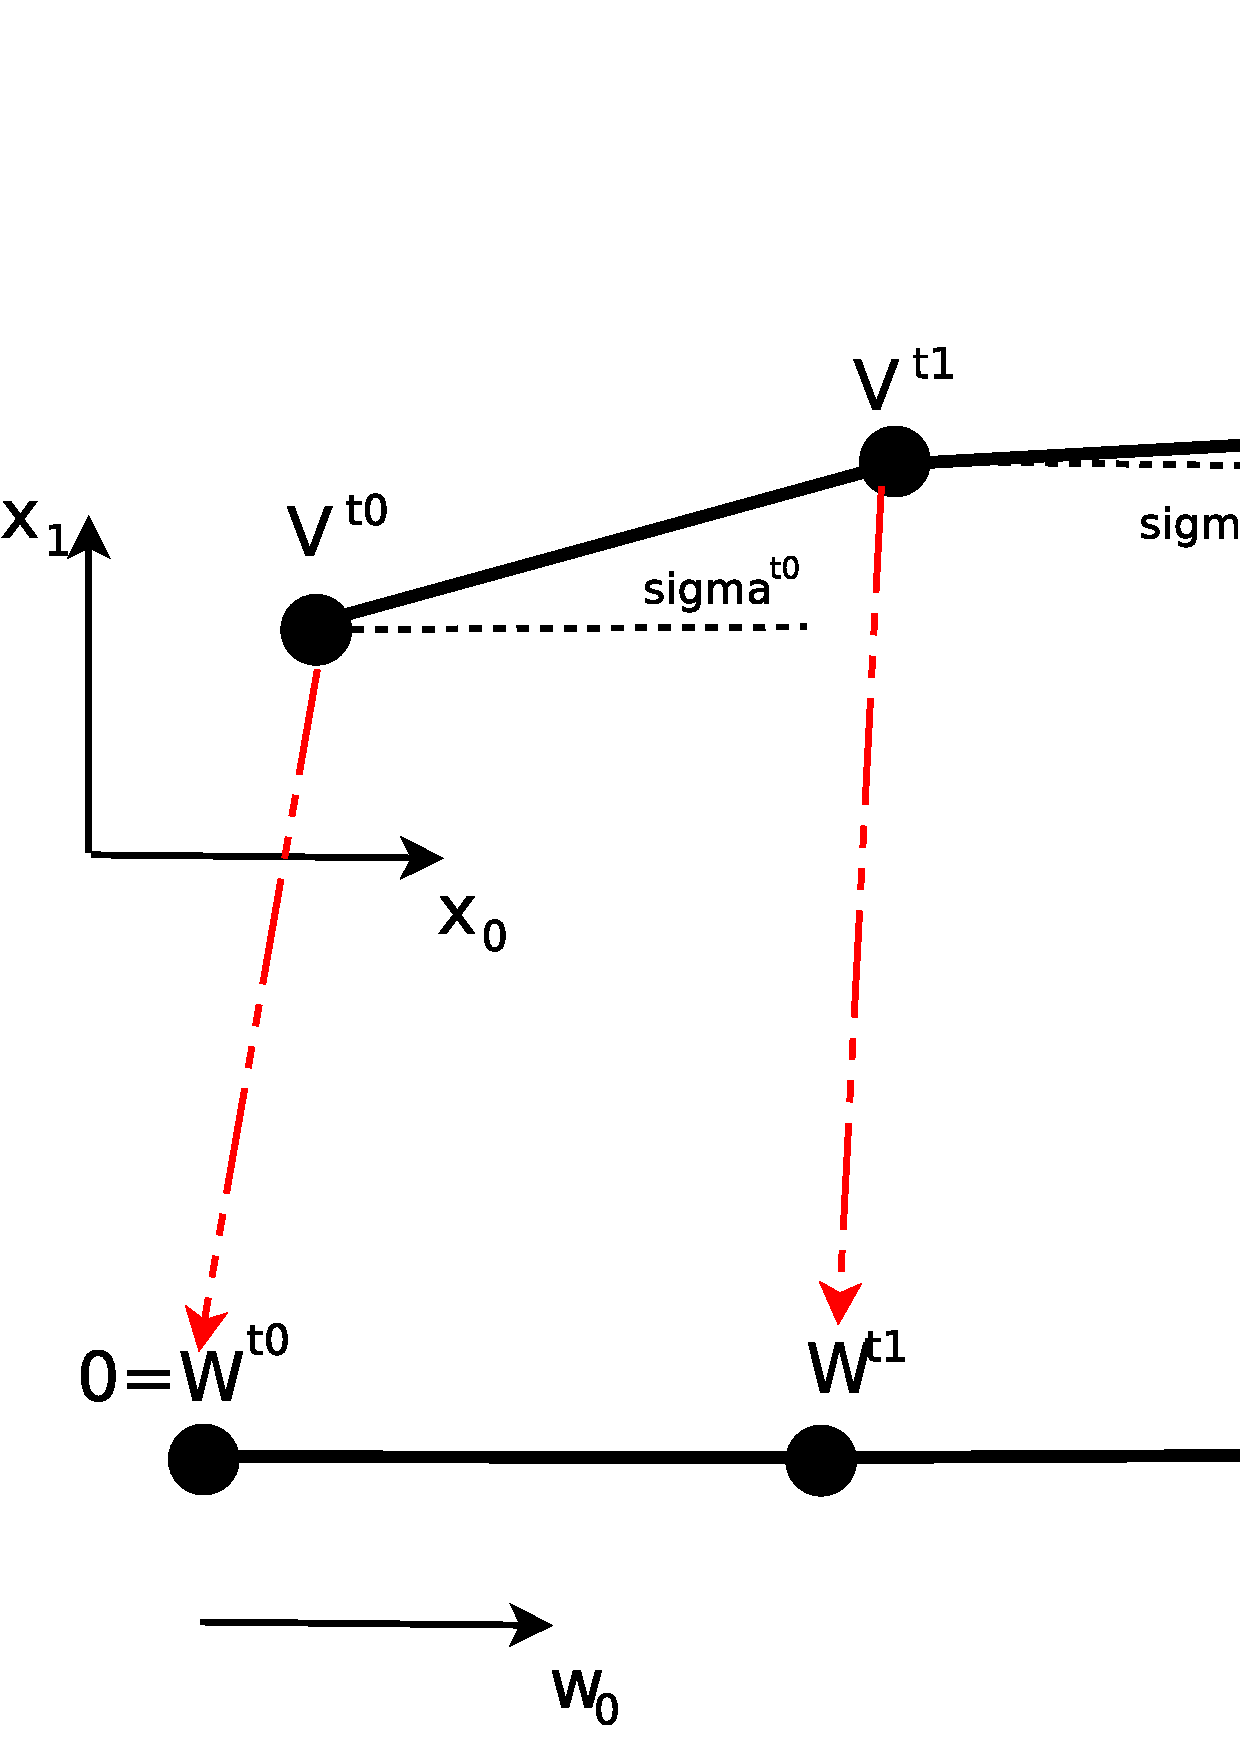
\includegraphics{FaultSystem2D}
\caption{\label{FAULTSYSTEM2D}Two dimensional fault system with one fault
named `t` in the $(x_{0},x_{1})$ space and its parameterization in the
$w_{0}$ space. The fault has three segments.}
\end{figure}

A fault $t$ in the fault system is represented by a starting point $V^{t0}$
and series of directions, called strikes\index{strike}, and the lengths $(l^{ti})$.
The strike of segment $i$ is defined by the angle $\sigma^{ti}$ between the
$x_{0}$-axis and the direction of the fault, see Figure~\ref{FAULTSYSTEM2D}.
The length and strike defines the polyline $(V^{ti})$ of the fault by
\begin{equation}
V^{ti} = V^{t(i-1)} + 
l^{ti} \cdot  S^{ti}
\mbox{ with }
S^{ti} =
\left[
\begin{array}{c}
 cos(\sigma^{ti})  \\
 sin(\sigma^{ti}) \\
 0 
\end{array}
\right]
\label{eq:fault 00}
\end{equation}
In the 3D case each fault segment $i$ has an additional dip\index{dip}
$\theta^{ti}$ and at each vertex $i$ a depth $\delta^{ti}$ is given.
The fault segment normal $n^{ti}$ is given by
\begin{equation}
n^{ti} = 
\left[
\begin{array}{c}
 -sin(\theta^{ti}) \cdot S^{ti}_{1} \\
 sin(\theta^{ti}) \cdot S^{ti}_{0} \\
 cos(\theta^{ti}) 
\end{array}
\right]
\label{eq:fault 0}
\end{equation}
At each vertex we define a depth vector $d^{ti}$ defined as the intersect of
the fault planes of segment $(i-1)$ and $i$ where for the first segment and
last segment the vector orthogonal to strike vector $S^{ti}$\index{strike}
and the segment normal $n^{ti}$ is used. The direction $\tilde{d}^{ti}$ of the
depth vector is given as
\begin{equation}
\tilde{d}^{ti} = n^{ti} \times n^{t(i-1)}
\label{eq:fault b}
\end{equation}
If $\tilde{d}^{ti}$ is zero the strike vectors $L^{t(i-1)}$ and $L^{ti}$ are
collinear and we can set $\tilde{d}^{ti} = l^{ti} \times n^{ti}$.
If the two fault segments are almost orthogonal $\tilde{d}^{ti}$ is pointing
in the direction of $L^{t(i-1)}$ and $L^{ti}$. In this case no depth can be
defined. So we will reject a fault system if
\begin{equation}
min(\| \tilde{d}^{ti}  \times  L^{t(i-1)} \|,\| \tilde{d}^{ti}  \times  L^{ti} \|) 
\le 0.1 \cdot \| \tilde{d}^{ti} | 
\label{eq:fault c}
\end{equation}
which corresponds to an angle of less than $10^o$ between the depth vector and
the strike. We then set
\begin{equation}
d^{ti}=\delta^{ti} \cdot \frac{\tilde{d}^{ti}}{\|\tilde{d}^{ti}\|}
\label{eq:fault d}
\end{equation}
We can then define the polyline $(v^{ti})$ for the bottom of the fault as
\begin{equation}
v^{ti}= V^{ti}+d^{ti}
\label{eq:fault e}
\end{equation}
In order to simplify working on a fault $t$ in a fault system a
parameterization $P^t: (w_{0},w_{1}) \rightarrow (x_{0},x_{1},x_{2})$ over a
rectangular domain is introduced such that
\begin{equation}
0\le w_{0} \le w^t_{0 max} \mbox{ and }  -w^t_{1max}\le w_{1} \le 0
\label{eq:fault 1}
\end{equation}
with positive numbers $w^t_{0 max}$ and $w^t_{1 max}$. Typically one chooses
$w^t_{0 max}$ to be the unrolled length of the fault and $w^t_{1 max}$ to be
the mean value of segment depth. Moreover we have
\begin{equation}
P^t(W^{ti})=V^{ti}\mbox{ and } P^t(w^{ti})=v^{ti}\
\label{eq:fault 2}
\end{equation}
where
\begin{equation}
W^{ti}=(\Omega^{ti},0) \mbox{ and } w^{ti}=(\Omega^{ti},-w^t_{1 max})
\label{eq:fault 3}
\end{equation}
and $\Omega^{ti}$ is the unrolled distance of $W^{ti}$ from $W^{t0}$, i.e.
$l^{ti}=\Omega^{t(i+1)}-\Omega^{ti}$. In the 2D case $w^t_{1 max}$ is set to
zero and therefore the second component is dropped, see Figure~\ref{FAULTSYSTEM2D}.

In the 2D case the parameterization $P^t$ is constructed as follows:
The line connecting $V^{t(i-1)}$ and $V^{ti}$ is given by
\begin{equation}
x=V^{ti} + s  \cdot  ( V^{t(i+1)}- V^{ti} )
\label{eq:2D line 1}
\end{equation}
where $s$ is between $0$ and $1$. The point $x$ is on $i$-th fault segment if
and only if such an $s$ exists. Assuming $x$ is on the fault it can be
calculated as
\begin{equation}
s = \frac{ (x- V^{ti})^t \cdot (V^{t(i+1)}- V^{ti}) }{ \|V^{t(i+1)}- V^{ti}\|^2} 
\label{eq:2D line 1b}
\end{equation}
We then can set
\begin{equation}
w_{0}=\Omega^{ti}+s \cdot (\Omega^{ti}-\Omega^{t(i-1)})
\label{eq:2D line 2}
\end{equation}
to get $P^t(w_{0})=x$.
It remains the question if the given $x$ is actually on the segment $i$ of
fault $t$. To test this $s$ is restricted between $0$ and $1$ (so if $s<0$, $s$
is set to $0$ and if $s>1$, $s$ is set to $1$) and then we check the residual
of \eqn{eq:2D line 1}, i.e. $x$ has been accepted to be in the segment if
\begin{equation}
\|x-V^{ti} - s \cdot (V^{t(i+1)}- V^{ti}) \| \le tol \cdot  
max(l^{ti}, \|x-V^{ti} \|) 
\label{eq:2D line 3}
\end{equation}
where $tol$ is a given tolerance.

In the 3D case the situation is a bit more complicated: we split the fault
segment across the diagonal $V^{ti}$-$v^{t(i+1)}$ to produce two triangles.
In the upper triangle we use the parameterization 
\begin{equation}
x= V^{ti} + s \cdot (V^{t(i+1)}-V^{ti})  + r \cdot (v^{t(i+1)}-V^{t(i+1)})
\mbox{ with } r \le s; 
\label{eq:2D line 4}
\end{equation}
while in the lower triangle we use
\begin{equation}
x= V^{ti} +  s \cdot (v^{t(i+1)}-v^{ti}) + r \cdot (v^{ti}-V^{ti})
\mbox{ with } s \le r; 
\label{eq:2D line 4b}
\end{equation}
where $0\le s,r \le 1$. Both equations are solved in the least-squares sense
e.g. using the Moore-Penrose pseudo-inverse for the coefficient matrices.
The resulting $s$ and $r$ are then restricted to the unit square. Similar to
the 2D case (see \eqn{eq:2D line 3}) we identify $x$ to be in the upper
triangle of the segment if
\begin{equation}
\|x- V^{ti} - s \cdot (V^{t(i+1)}-V^{ti})  - r \cdot (v^{t(i+1)}-V^{t(i+1)}) \|
\le tol \cdot  max(\|x-V^{ti} \|,\|v^{t(i+1)}-V^{t(i)})\|) 
\label{eq:2D line 4c}
\end{equation}
and in the lower part
\begin{equation}
\|x-V^{ti} -  s \cdot (v^{t(i+1)}-v^{ti}) - r \cdot (v^{ti}-V^{ti}) \|
\le tol \cdot  max(\|x-V^{ti} \|,\|v^{t(i+1)}-V^{t(i)})\|)  
\label{eq:2D line 4d}
\end{equation}
after the restriction of $(s,t)$ to the unit square.
Note that $\|v^{t(i+1)}-V^{t(i)})\|$ is the length of the diagonal of the
fault segment. For those $x$ which have been located in the $i$-th segment we
then set
\begin{equation}
w_{0}=\Omega^{ti}+s \cdot (\Omega^{ti}-\Omega^{t(i-1)})
\mbox{ and }
w_{1}=w^t_{1max} (r-1) 
\label{eq:2D line 5}
\end{equation}

\subsection{Functions}

\begin{classdesc}{FaultSystem}{\optional{dim =3}}
creates a fault system in the \var{dim} dimensional space.
\end{classdesc}

\begin{methoddesc}[FaultSystem]{getMediumDepth}{tag}
returns the medium depth of fault \var{tag}.
\end{methoddesc}

\begin{methoddesc}[FaultSystem]{getTags}{}
returns a list of the tags used by the fault system.
\end{methoddesc}

\begin{methoddesc}[FaultSystem]{getStart}{tag}
returns the starting point of fault \var{tag} as a \numpyNDA object.
\end{methoddesc}

\begin{methoddesc}[FaultSystem]{getDim}{}
returns the spatial dimension.
\end{methoddesc}

\begin{methoddesc}[FaultSystem]{getDepths}{tag}
returns the list of the depths of the segments in fault \var{tag}.
\end{methoddesc}

\begin{methoddesc}[FaultSystem]{getTopPolyline}{tag}
returns the polyline used to describe the fault tagged by \var{tag}.
\end{methoddesc}

\begin{methoddesc}[FaultSystem]{getStrikes}{tag}
returns the list of strikes $\sigma^{ti}$ of the segments in fault
$t=$\var{tag}.
\end{methoddesc}

\begin{methoddesc}[FaultSystem]{getStrikeVectors}{tag}
returns the strike vectors $S^{ti}$ of fault $t=$\var{tag}.
\end{methoddesc}

\begin{methoddesc}[FaultSystem]{getLengths}{tag}
returns the lengths $l^{ti}$ of the segments in fault $t=$\var{tag}.
\end{methoddesc}

\begin{methoddesc}[FaultSystem]{getTotalLength}{tag}
returns the total unrolled length of fault \var{tag}.
\end{methoddesc}

\begin{methoddesc}[FaultSystem]{getDips}{tag}
returns the list of the dips of the segments in fault \var{tag}.
\end{methoddesc}

\begin{methoddesc}[FaultSystem]{getBottomPolyline}{tag}
returns the list of the vertices defining the bottom of the fault \var{tag}.
\end{methoddesc}

\begin{methoddesc}[FaultSystem]{getSegmentNormals}{tag}
returns the list of the normals of the segments in fault \var{tag}.
\end{methoddesc}

\begin{methoddesc}[FaultSystem]{getDepthVectors}{tag}
returns the list of the depth vectors $d^{ti}$ for fault $t=$\var{tag}.
\end{methoddesc}

\begin{methoddesc}[FaultSystem]{getDepths}{tag}
returns the list of the depths of the segments in fault \var{tag}.
\end{methoddesc}

\begin{methoddesc}[FaultSystem]{getW0Range}{tag}
returns the range of the parameterization in $w_{0}$.
For tag $t$ this is the pair $(\Omega^{t0},\Omega^{tn})$ where $n$ is the
number of segments in the fault.
In most cases one has $(\Omega^{t0},\Omega^{tn})=(0,w^t_{0 max})$.
\end{methoddesc}

\begin{methoddesc}[FaultSystem]{getW1Range}{tag}
returns the range of the parameterization in  $w_{1}$.
For tag $t$ this is the pair $(-w^t_{1max},0)$.
\end{methoddesc}

\begin{methoddesc}[FaultSystem]{getW0Offsets}{tag}
returns the offsets for the parameterization of fault \var{tag}.
For tag \var{tag}=$t$ this is the list $[\Omega^{ti}]$.
\end{methoddesc}

\begin{methoddesc}[FaultSystem]{getCenterOnSurface}{}
returns the center point of the fault system at the surfaces.
In 3D the calculation of the center is considering the top edge of the faults
and projects the edge to the surface (the $x_{2}$ component is assumed to be
0). An \numpyNDA object is returned.
\end{methoddesc}

\begin{methoddesc}[FaultSystem]{getOrientationOnSurface}{}
returns the orientation of the fault system in RAD on the surface
($x_{2}=0$ plane) around the fault system center.
\end{methoddesc}

\begin{methoddesc}[FaultSystem]{transform}{\optional{rot=0, \optional{shift=numpy.zeros((3,)}}}
applies a shift \var{shift} and a consecutive rotation in the $x_{2}=0$ plane.
\var{rot} is a float number and \var{shift} an \numpyNDA object.
\end{methoddesc}

\begin{methoddesc}[FaultSystem]{getMaxValue}{f\optional{, tol=1.e-8}}
returns the tag of the fault where \var{f} takes the maximum value and a
\class{Locator} object which can be used to collect values from \Data objects
at the location where the maximum is taken, e.g.
\begin{python}
       fs=FaultSystem()
       f=Scalar(..)
       t, loc=fs.getMaxValue(f)
       print("maximum value of f on the fault %s is %s at location %s."%(t, \
             loc(f), loc.getX()))
\end{python}
\var{f} must be a \Scalar. When the maximum is calculated only
\DataSamplePoints are considered which are on a fault in the fault system in
the sense of condition~\ref{eq:2D line 3} or \ref{eq:2D line 4d}, respectively.
In the case no \DataSamplePoints are found the returned tag is \var{None} and
the maximum value as well as the location of the maximum value are undefined.
\end{methoddesc}

\begin{methoddesc}[FaultSystem]{getMinValue}{f\optional{, tol=1.e-8}}
returns the tag of the fault where \var{f} takes the minimum value and a
\class{Locator} object which can be used to collect values from \Data objects
at the location where the minimum is taken, e.g.
\begin{python}
  fs=FaultSystem()
  f=Scalar(..)
  t, loc=fs.getMinValue(f)
  print("minimum value of f on the fault %s is %s at location."%(t,loc(f),loc.getX()))
\end{python}
\var{f} must be a \Scalar. When the minimum is calculated only
\DataSamplePoints are considered which are on a fault in the fault system in
the sense of condition~\ref{eq:2D line 3} or \ref{eq:2D line 4d}, respectively.
In the case no \DataSamplePoints are found the returned tag is \var{None} and
the minimum value as well as the location of the minimum value are undefined.
\end{methoddesc}

\begin{methoddesc}[FaultSystem]{getParametrization}{x,tag \optional{\optional{, tol=1.e-8}, outsider=None}}
returns the argument $w$ of the parameterization $P^t$ for \var{tag}=$t$ to
provide \var{x} together with a mask indicating where the given location if on
a fault in the fault system by the value $1$ (otherwise the value is set to $0$).
\var{x} needs to be a \Vector or \numpyNDA object.
\var{tol} defines the tolerance to decide if given \DataSamplePoints are on
fault \var{tag}. The value \var{outside} is the value used as a replacement
value for $w$ where the corresponding value in \var{x} is not on a fault.
If \var{outside} is not present an appropriate value is used.
\end{methoddesc}
 
\begin{methoddesc}[FaultSystem]{getSideAndDistance}{x,tag}
returns the side and the distance at locations \var{x} from the fault \var{tag}.
\var{x} needs to be a \Vector or \numpyNDA object.
Positive values for side means that the corresponding location is to the right
of the fault, a negative value means that the corresponding location is
to the left of the fault. The value zero means that the side is undefined.
\end{methoddesc}

\begin{methoddesc}[FaultSystem]{getFaultSegments}{tag}
returns the polylines used to describe fault \var{tag}. For \var{tag}=$t$ this
is the list of the vertices $[V^{ti}]$ for the 2D and the pair of lists of the
top vertices $[V^{ti}]$ and the bottom vertices $[v^{ti}]$ in 3D.
Note that the coordinates are represented as \numpyNDA objects.
\end{methoddesc}

\begin{methoddesc}[FaultSystem]{addFault}{
strikes\optional{,
ls\optional{,
V0=[0.,0.,0.]\optional{,
tag=None\optional{,
dips=None\optional{,
depths= None\optional{,
w0_offsets=None\optional{,
w1_max=None}}}}}}}}
adds the fault \var{tag} to the fault system.
\var{V0} defines the start point of fault named $t=$\var{tag}.
The polyline defining the fault segments on the surface are set by the strike
angles \var{strikes} (=$\sigma^{ti}$, north = $\pi/2$, the orientation is
counterclockwise.) and the length \var{ls} (=$l^{ti}$).
In the 3D case one also needs to define the dip angles \var{dips}
(=$\delta^{ti}$, vertical=$0$, right-hand rule applies.) and the depth
\var{depths} for each segment.
\var{w1_max} defines the range of $w_{1}$.
If not present the mean value over the depth of all segment edges in the fault
is used.
\var{w0_offsets} sets the offsets $\Omega^{ti}$. If not present it is chosen
such that $\Omega^{ti}-\Omega^{t(i-1)}$ is the length of the $i$-th segment.
In some cases, e.g. when kinks in the fault are relevant, it can be useful
to explicitly specify the offsets in order to simplify the assignment of values.
\end{methoddesc}

\subsection{Example}
See \Sec{Slip CHAP}.



% \section{Drucker Prager Model}